%%% Local Variables:
%%% TeX-command-extra-options: "-shell-escape"
%%% mode: latex
%%% TeX-master: t
%%% End:
\documentclass{beamer}
\usepackage{caption}
\usepackage{minted}
\usepackage{tikz}
\usepackage{xcolor}
\usetikzlibrary{shapes.geometric, arrows}
\tikzstyle{startstop} = [rectangle, rounded corners, minimum width=3cm, minimum height=1cm,text centered, draw=black, fill=red!30]
\tikzstyle{io} = [trapezium, trapezium left angle=70, trapezium right angle=110, minimum width=1.5cm, minimum height=0.6cm, text centered, draw=black, fill=blue!30]
\tikzstyle{process} = [rectangle, minimum width=1.5cm, minimum height=0.5cm, text centered, draw=black, fill=orange!30]
\tikzstyle{decision} = [circle, radius=2.5cm, text centered, draw=black, fill=green!30]
\tikzstyle{arrow} = [thick,->,>=stealth]
\usepackage[labelformat=simple]{subcaption}

\usetheme{Singapore}
\title{Abstraction}

\begin{document}
\begin{frame}
\titlepage
\end{frame}
\section{Abstract Nonsense}

\begin{frame}
  \huge \centering \url{https://en.wikipedia.org/wiki/Abstract_nonsense}
\end{frame}

\begin{frame}
  \frametitle{Software Engineers and Patterns}
  \centering 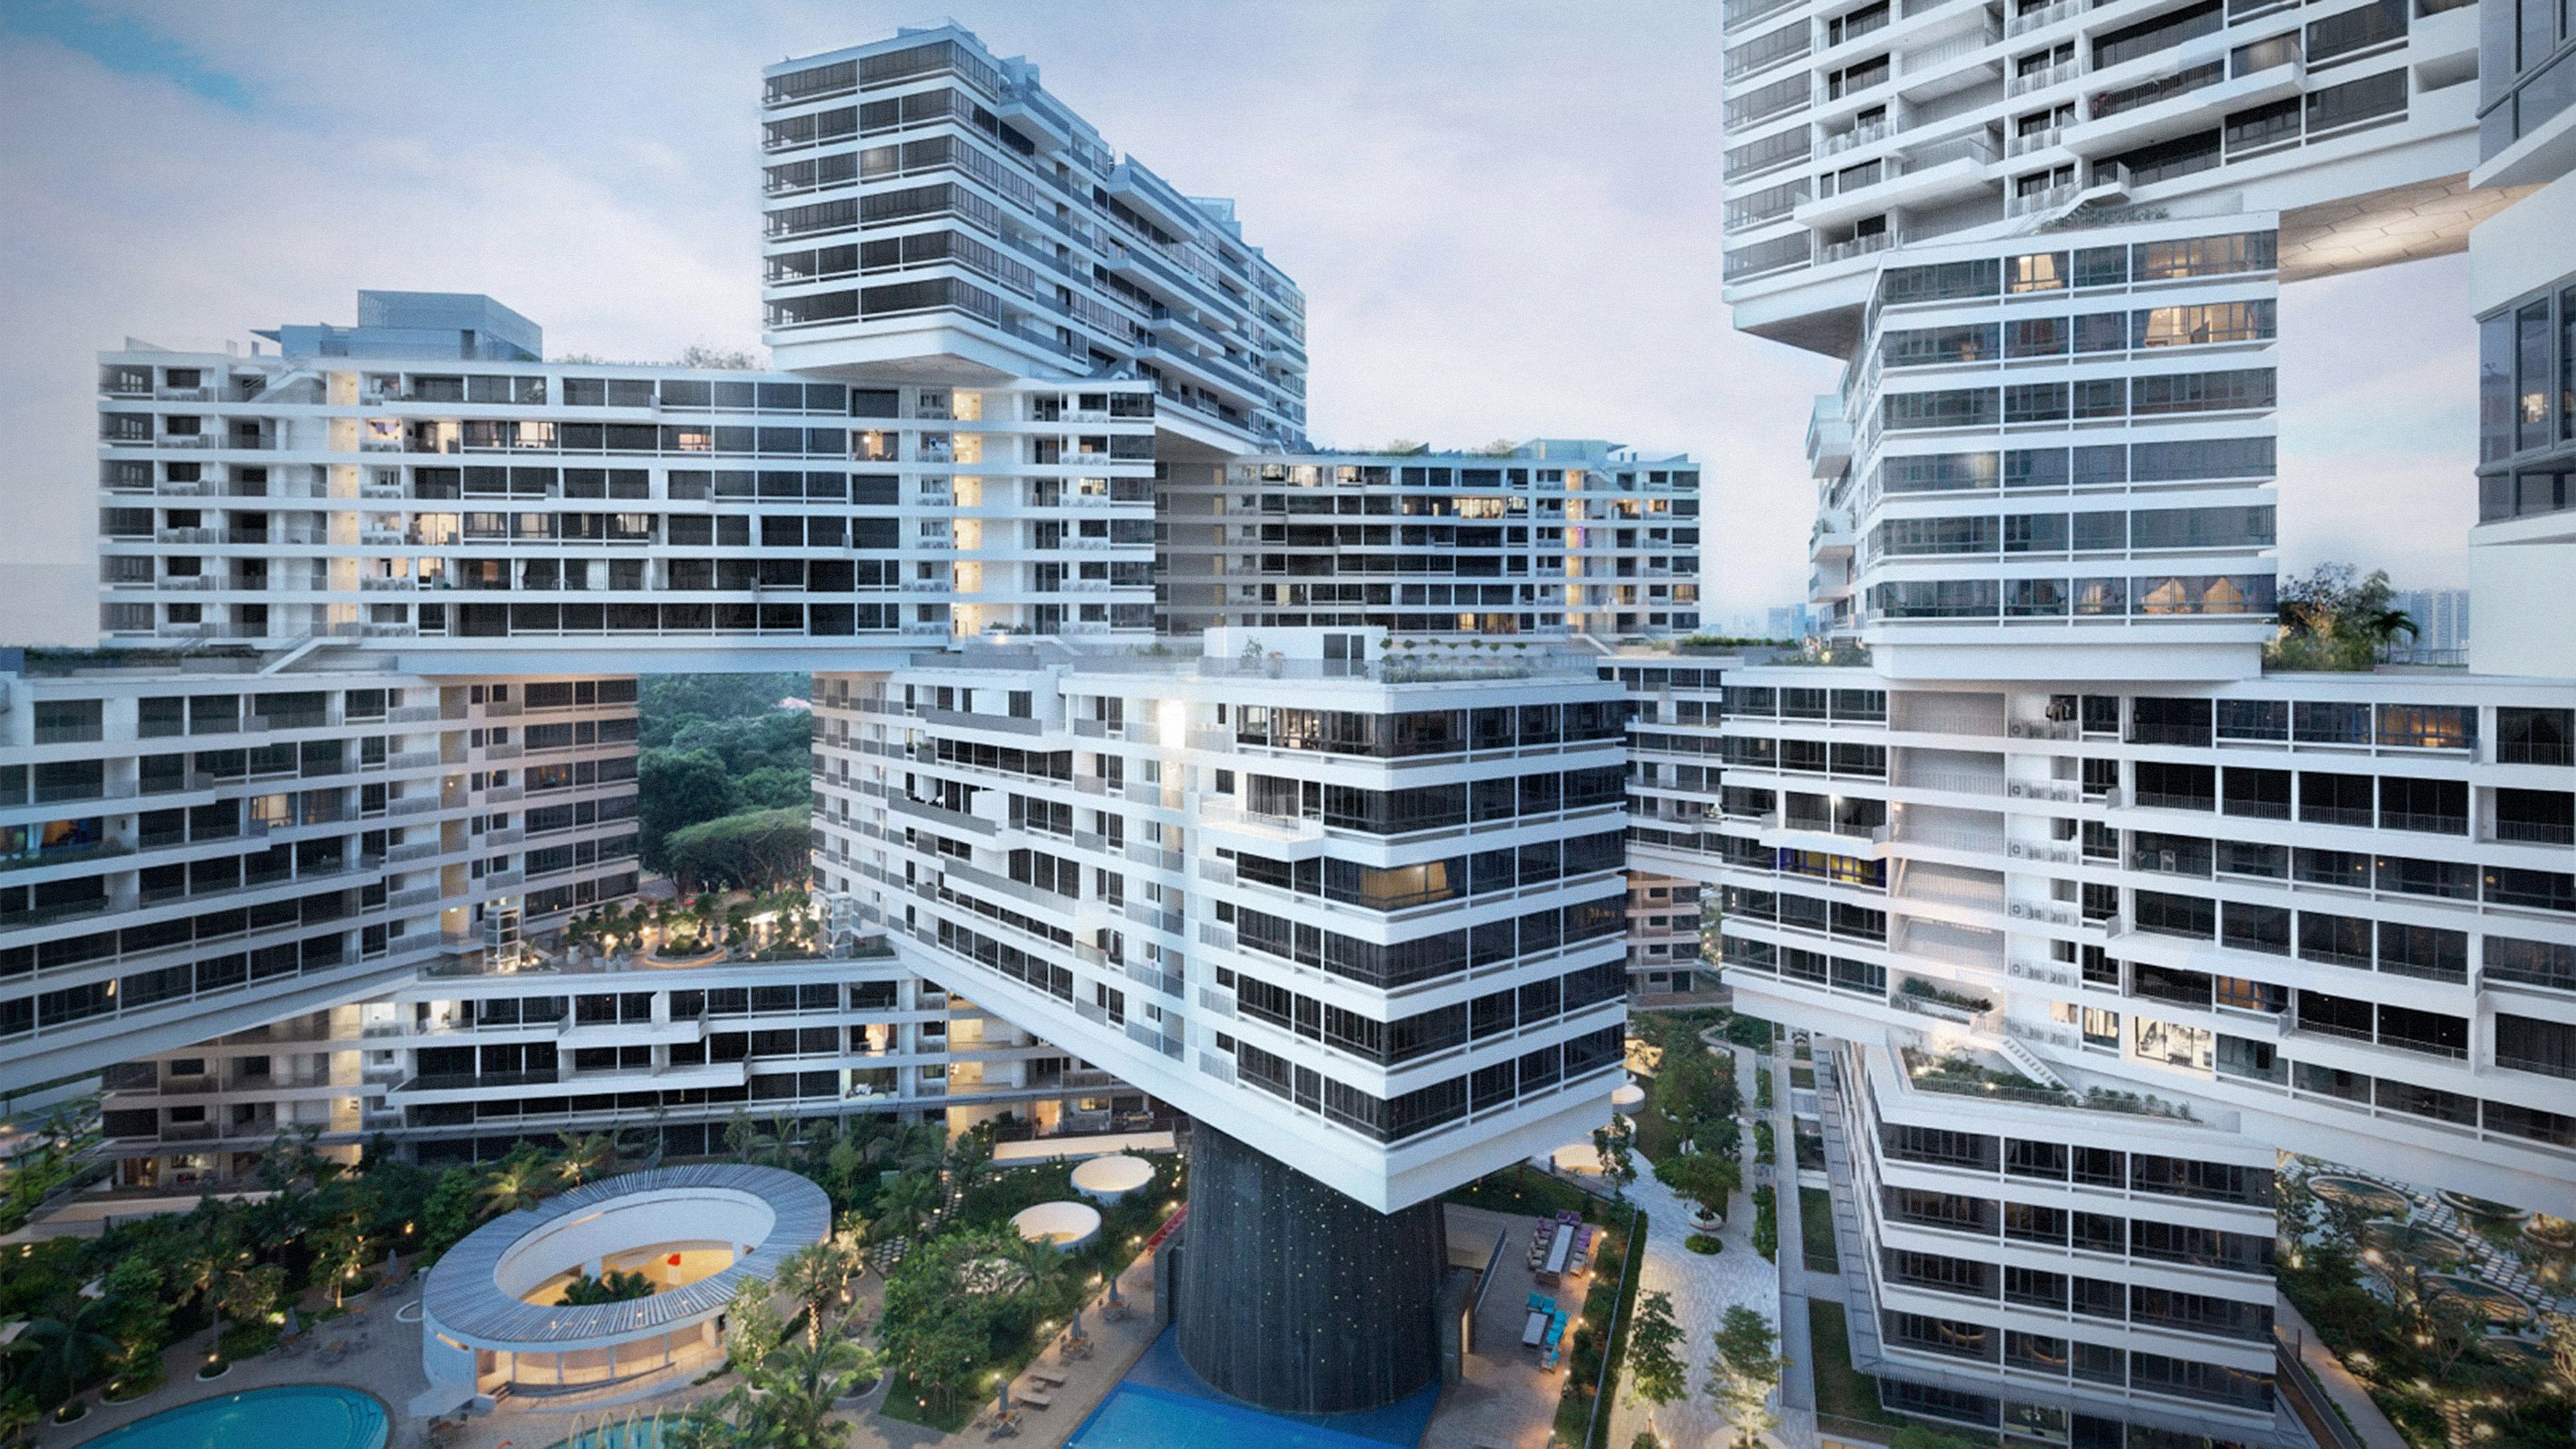
\includegraphics[width=0.3\textwidth]{images/architecture.jpg}
  \begin{itemize}
  \item<2-> Software engineers love architecture principles.
  \item<3-> Who has heard of \emph{design patterns} and the gang of four book?
  \item<4-> The authors were actually inspired by a book that came up with
    a pattern language in architecture
  \item<5-> Such patterns were meant to provide guidelines across buildings in multiple
    style \emph{abstracting} away concrete details of individual buildings.
  \item<6-> Software design patterns are thus all about providing \emph{abstractions}.
  \end{itemize}
\end{frame}

\begin{frame}
  \frametitle{Theories of Abstraction}
  Let's talk about abstraction.
  \begin{itemize}
  \item<2-> 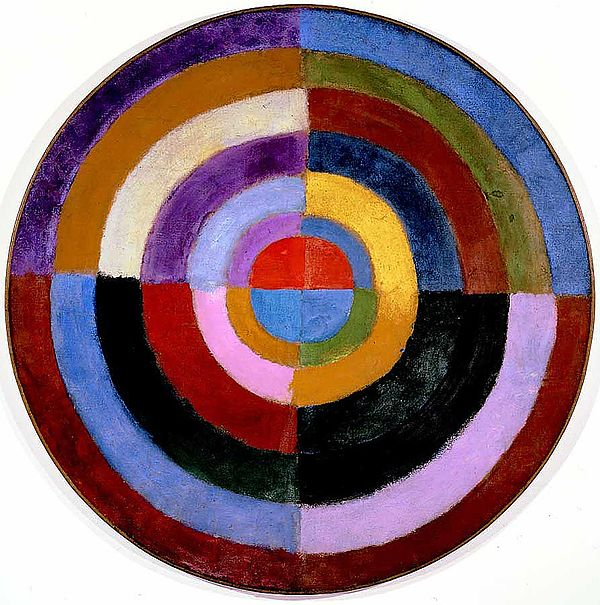
\includegraphics[width=0.3\textwidth]{images/abstract-art.jpg}
  \item<3-> Abstraction in visual
    art is about avoiding concrete subjects. It attempts
    to convey something (often an emotion) without appealing to sentiment.
  \item<4-> Oddly enough there's a bit of a stigma against it, despite the
    fact that music without lyrics has far less stigma.
  \item<5-> Abstraction in mathematics and computer science is about
    \emph{generalization}. Take away the concrete details of certain objects
    and see how they are similar.
  \end{itemize}
\end{frame}

\begin{frame}
  \frametitle{Why Abstract?}
  This can lead us to \emph{classify} different objects into
    related groups.
  \begin{itemize}
  \item<2-> Category theory has been influential in programming language theory
    because it is a powerful language for communicating abstractions in ways
    that are largely \emph{constructive}.
  \item<3-> This is important to computing because the point of programs
    are to construct some form of answer.
  \item<4-> Although categorical abstractions are powerful, I will not discuss them much (and most of the really powerful abstractions go over my head).
  \item<5-> But we will study abstraction from a less mathematical viewpoint.
  \item<6-> I will show instances of \emph{almost identical} code and how a programming language feature allows the two pieces of code to be generalized. 
  \end{itemize}    
\end{frame}

\defverbatim[colored]\buddies{
\begin{minted}[fontsize=\footnotesize]{Java}
  public boolean hasSmith(List<String> names) {
    for (String name : names) {
      if (name == "Smith")
        return true;
    }
    return false;
  }

  public  boolean hasBob(List<String> names) {
    for (String name : names) {
      if (name == "Bob")
        return true;
    }
    return false;
  }
\end{minted}
}

\begin{frame}
  \frametitle{Buddy Functions}
  Let's consider the following functions in Java:
  \buddies
  \pause
  These look pretty similar, right?
\end{frame}

\defverbatim[colored]\abstractOne{
\begin{minted}[fontsize=\footnotesize]{Java}
  public boolean hasName(String searchName, List<String> names) {
    for (String name : names) {
      if (name == searchName)
        return true;
    }
    return false;
  }
\end{minted}
}

\begin{frame}
  \frametitle{Eliminate Redundancy!}
  So, let's eliminate the redundancy of searching
  for different names by abstracting out towards
  a definition that takes in a string parameter
  to search for. This generalizes writing functions
  to search for specific strings.

  \abstractOne
  \begin{itemize}
  \item<2-> Why only design a function that searches for names?
  \item<3-> Why not search for arbitrary items so long as they
    are comparable?
  \item<4-> Then searching for names becomes an instance of a
    more general problem that is solved.    
  \end{itemize}
\end{frame}

\defverbatim[colored]\abstractTwo{
\begin{minted}[fontsize=\footnotesize]{Java}
  public <T extends Comparable<T>>
    boolean hasItem(T searchItem, List<T> items) {
    for (T item : items) {
      if (item.equals(searchItem))
        return true;
    }
    return false;
  }
\end{minted}
}

\begin{frame}
  \frametitle{Generic Structure}
  So, let's use some Java \emph{generics} to generalize our program.
  \abstractTwo
  \begin{itemize}
  \item<2-> Alright, now we can search for arbitrary comparable items!
  \item<3-> This is nice and general!
  \item<4-> Can we generalize any more?
  \item<5-> We actually have 2 more abstractions that we can apply!
  \end{itemize}
\end{frame}

\begin{frame}
  \frametitle{Two Abstractions??}
  \centering 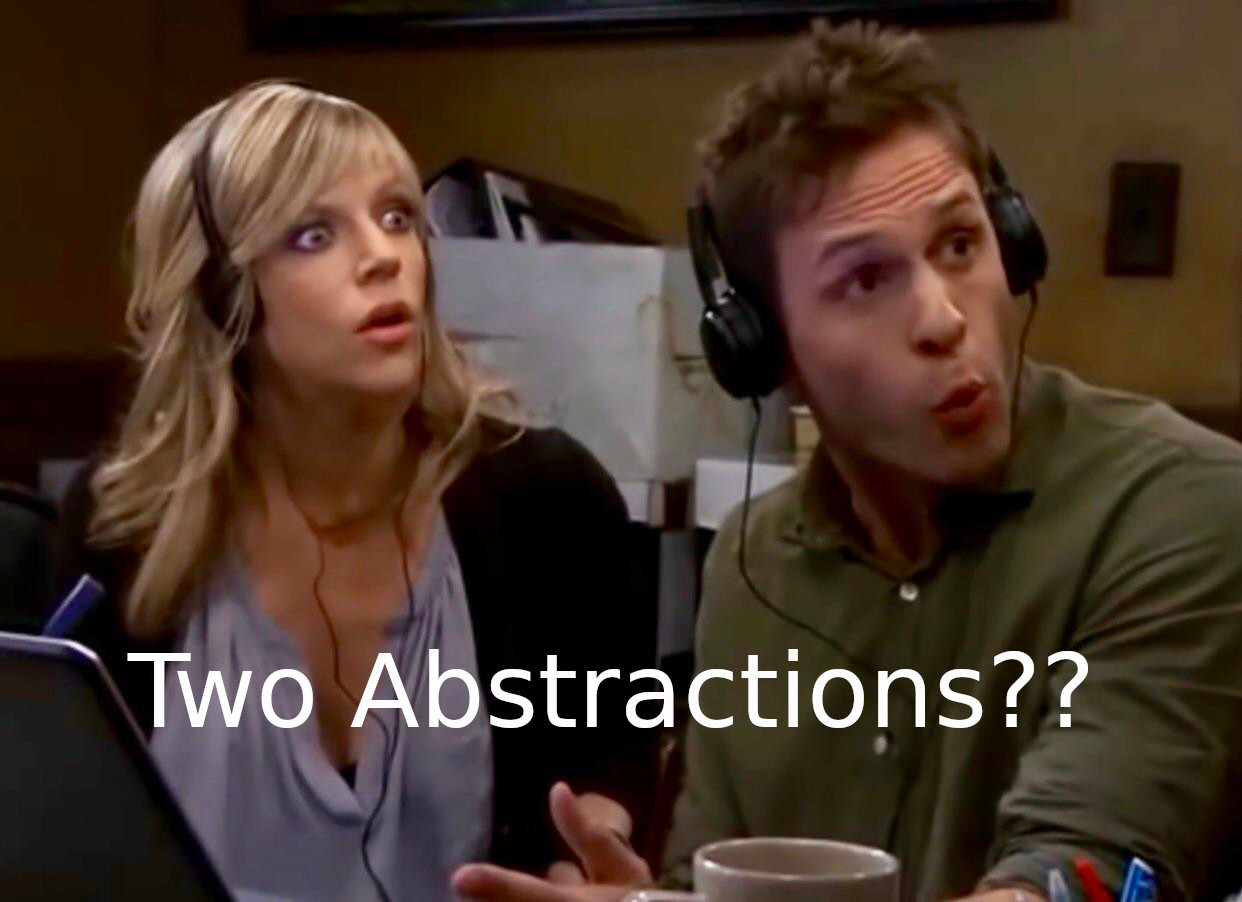
\includegraphics[width=0.6\textwidth]{images/two-abstractions.jpg}
\end{frame}

\begin{frame}
  \frametitle{I'm Sorry}
  \centering 
\includegraphics[width=0.6\textwidth]{images/unnecessary.png}
\end{frame}

\defverbatim[colored]\abstractThree{
\begin{minted}[fontsize=\footnotesize]{Java}
  public <T extends Comparable<T>>
    boolean testItems(Predicate<T> pred, List<T> items) {
    for (T item : items) {
      if (pred.test(searchItem))
        return true;
    }
    return false;
  }
\end{minted}
}

\begin{frame}
  \frametitle{Back on Track}
  Ok, let's get down to business.
  \begin{itemize}
  \item<2-> 
\includegraphics[width=0.3\textwidth]{images/business.png}
  \item<3-> We can actually consider searching for a specific item via equality
    as the process of seeing if an arbitrary predicate returns true for an item
    in a list.
  \item<4-> So if we wanted to check if a string equaled smith we could write:
    \mintinline{Java}{Predicate<String> isSmith = str -> str == "Smith";}
  \item<5-> I could then pass this as the first argument to a funciton \mintinline{Java}{TestItems}
    that I will now define.
  \end{itemize}
\end{frame}

\defverbatim[colored]\abstractFour{
\begin{minted}[fontsize=\footnotesize]{Java}
  public <T extends Comparable<T>>
    boolean testItems(Predicate<T> pred, Iterable<T> items) {
      for (T item : items) {
        if (pred.test(item))
          return true;
      }
      return false;
    }
\end{minted}
}

\begin{frame}
  \frametitle{Last Abstraction}
  Here is that function now:
  \abstractThree
  \begin{itemize}
  \item<2-> We can provide one last abstraction that applies predicates to every item in \emph{any iterable collection}.
  \item<3-> For example, if I define iterators over dictionaries or trees we should still be able to
    apply a predicate to them.
  \item<4-> \abstractFour
  \end{itemize}
\end{frame}

\begin{frame}
  \frametitle{Predicates as Arguments}
  Our third abstraction was a bit strange, right?
  \begin{itemize}
  \item<2-> I used this weird predicate type in Java and then assigned an \emph{anonymous function}.
  \item<3-> This is a function with no name, and it is useful if you only need to use a function
    in one place in your program.
  \item<4-> The second thing is that we had a parameter that received a function as input.
  \item<5-> It then applied this function to every element in the list and observed whether it
    returned \mintinline{Java}{true} for that element.
  \item<6-> This is a very powerful concept where we can determine if perhaps all elements in a collection
    satisfy a property or even one element. Or we can collect all individuals in a collection that satisfy
    some property.
  \item<7-> For example, let's consider writing a program that only admits people that are 18 and older. 
  \end{itemize}
\end{frame}

\defverbatim[colored]\BarEntry{
\begin{minted}[fontsize=\footnotesize]{racket}
  ;; List<Person> -> List<Person>
  ;; Only allows patrons over 18 to enter the bar
  (define (bar-entry patrons)
    (cond
      [(empty? patrons) patrons]
      [(cons? patrons)
         (... (first patrons)) ... (bar-entry (rest patrons))]))  
\end{minted}
}

\begin{frame}
  \frametitle{Guarding Entry}
  Let's consider that we have a list of people whose ages are represented by Natural numbers and that we want to only collect the people
  over 18. Assume a person has an age field that we can project.
  \begin{itemize}
  \item<2-> How do we start writing such a function?
  \item<3-> Via recursion over a list of course.
  \item<4-> I'll skip to providing a skeleton:
  \item<5-> \BarEntry
  \end{itemize}
\end{frame}

\begin{frame}
  \frametitle{Guarding Entry}
  So, in order to protect against underage patrons getting in, we must do a comparision.
  \begin{itemize}
  \item<2-> Assume that \mintinline{racket}{(first patrons)} returns \mintinline{racket}{(person "Sara" 26)}.
  \item<3-> How do I get the age out?
  \item<4-> \mintinline{racket}{(person-age (first patrons))}
  \item<5-> How do I check whether the age is less than 18?
  \item<6-> \mintinline{racket}{(< (person-age (first patrons)) 18)}
  \item<7-> Thus, we should get \mintinline{racket}{(< 26 18)} since we are getting Sara as our person,
    and this should return false.
  \item<8-> Since this returns false, we should throw Sara into the list we're building. How do we do that?
  \item<9-> With \mintinline{racket}{(cons (first patrons) ...)}  
  \end{itemize}
\end{frame}

\begin{frame}
  \frametitle{Only Collecting \emph{Some} Items}
  But what if \mintinline{racket}{(first patrons)} returns \mintinline{racket}{(person "Dustin" 16)}?
  \begin{itemize}
  \item<2-> Then, we had \mintinline{racket}{(< (person-age (person "Dustin" 16)) 18)}
  \item<3-> which evaluates to \mintinline{racket}{(< 16 18)} and then return true.
  \item<4-> This means that we must not add Dustin to our patron list. So we shouldn't use a cons operation.
  \item<5-> There are two ways around this. One is to locally add a complicated if expression. The second is to design
    a new function that only does a cons operation if the first element of the list has an age greater than 18 and otherwise
    returns the sublist that already had filtered out underage people.
  \item<6-> Let's consider designing this second function, called \mintinline{racket}{cons-over-18}
  \item<7-> Does this function need to do recursion itself?
  \end{itemize}
\end{frame}

\defverbatim[colored]\ConsOver{
\begin{minted}[fontsize=\footnotesize]{racket}
    ;; List<person> -> List<person>
    ;; Add a person to the patron list as
    ;; long as they are over 18.
    (define (cons-over-18 possible-patron patrons)
      (if (>= (person-age possible-patron) 18)
          (cons possible-patron patrons)
          patrons))  
\end{minted}
}

\begin{frame}
  \frametitle{Designing a Helper Function}
  Thankfully, our helper function does not need to do recursion!
  \begin{itemize}
  \item<2-> Why?
  \item<3-> We assume that the recursion for \mintinline{racket}{bar-entry} already filters out people from sublists.
  \item<4-> So, our helper function simply takes in a person and a list
    and only conses the person onto the list if they are over 18.
  \item<5-> \ConsOver
  \end{itemize}
\end{frame}

\defverbatim[colored]\BarFinal{
\begin{minted}[fontsize=\footnotesize]{racket}
  ;; List<Person> -> List<Person>
  ;; Only allows patrons over 18 to enter the bar
  (define (bar-entry patrons)
    (cond
      [(empty? patrons) patrons]
      [(cons? patrons)
         (cons-over-18 (first patrons) (bar-entry (rest patrons)))]))    
\end{minted}
}

\begin{frame}
  \frametitle{Finishing Our Bouncer Program}
  Alright, with our helper combinator we can structure our recursive function
  in the usual way, instead of having to add an additional condition in the
  body of the function.
  \begin{itemize}
  \item<2-> \BarFinal
  \item<3-> In general, if it seems like the list you're building depends
    on the structure of the values in the list, then you need some kind
    of cons operation that checks properties on the head of the list.
  \item<4-> But what happens if the condition we are checking needs to change?
  \end{itemize}
\end{frame}

\defverbatim[colored]\BarComplex{
  \begin{minted}[fontsize=\footnotesize]{racket}
    (define (cons-over-18 possible-patron patrons)
      (if (>= (person-age possible-patron) 18)
          (cons possible-patron patrons)
          patrons))
    (define (bar-entry-18 patrons)
      (cond
        [(empty? patrons) patrons]
        [(cons? patrons) (cons-over-18
                           (first patrons)
                           (bar-entry-18 (rest patrons)))]))
    (define (cons-over-21 possible-patron patrons)
      (if (>= (person-age possible-patron) 21)
           (cons possible-patron patrons)
           patrons))
    (define (bar-entry-21 patrons)
      (cond
        [(empty? patrons) patrons]
        [(cons? patrons) (cons-over-21
                          (first patrons)
                          (bar-entry-21 (rest patrons)))]))
  \end{minted}
}

\begin{frame}
  \frametitle{Adjusting Our Bouncer Program}
  Concretely, let's say that that our bar was serving alcohol to
    patrons under 21 (this is illegal but common...) and a new Sheriff comes in
    and is stricter on enforcing alcohol laws.
    \begin{itemize}
  \item<2-> Now our bar can't afford to give drinks to patrons under 21 years old.
    We decide that the easiest solution is to only allow 21 and over patrons,
    to prevent underage people from getting in and sneakily get drinks.
  \item<3-> To model this behavior, our program must change
    \mintinline{racket}{cons-over-18} to something named \mintinline{racket}{cons-over-21} that changes its check to make sure patrons are at least 21.
  \item<4-> But let's say we still need to model another bar that allows people over 18, but charges them covers. Then we will need four functions for our program.  
  \end{itemize}
\end{frame}

\begin{frame}
  \frametitle{Repetitive Bar Program}
  \BarComplex
\end{frame}

\begin{frame}
  \frametitle{How to Eliminate Redundant Code?}
  So, we can see we have a lot of redundant code in the program.
  \begin{itemize}
  \item<2-> Redundant code should cause developers an itch.
  \item<3-> On the one hand, there are more places for the program
    to go wrong.
  \item<4-> On the other, most developers get bored of re-reading similar code.
  \item<5-> To minimize failure locations and keep interest, we should
    \emph{abstract} out patterns in the code.
  \item<6-> So, how do we get started?
  \end{itemize}
\end{frame}

\defverbatim[colored]\BarAbstracted{
  \begin{minted}[fontsize=\footnotesize]{racket}
    (define (cons-over age possible-patron patrons)
      (if (>= (person-age possible-patron) age)
          (cons possible-patron patrons)
          patrons))
    (define (bar-entry age patrons)
      (cond
        [(empty? patrons) patrons]
        [(cons? patrons) (cons-over age
                           (first patrons)
                           (bar-entry (rest patrons)))]))
  \end{minted}
}

\begin{frame}
  \frametitle{Adding Parameters}
  A rule of thumb when abstracting code is that either you need
  another parameter or you need another function.
  \begin{itemize}
  \item<2-> Let's consider adding another parameter. We can add a boolean parameter that is a flag indicating
    whether to check if patrons are over 18 if the flag is false and over
    21 if it is true.
  \item<4-> But wouldn't it be more elegant to just have a numeric parameter
    that is used as the threshold for our checks?
  \item<5-> 
    \BarAbstracted
  \end{itemize}
\end{frame}

\begin{frame}
  \frametitle{What if We Need More Restrictions?}
  Now, let's say that we need to check that patrons have a valid id that
  hasn't expired. Assume that our persons struct has been updated with id
  information.
  \begin{itemize}
  \item<2-> How do we have to change to our program to account for this new
    restriction?
  \item<3-> We need to change \mintinline{racket}{cons-over} to add an additional
    check.
  \item<4-> Luckily, this restriction applies to all bars, so we don't have to
    add an additional parameter.
  \item<5-> But in general, as we add restrictions, we have to keep modifying
    \mintinline{racket}{cons-over}.
  \item<6-> Is there any way we can abstract over these changes?
  \item<7-> Just like the abstraction I provided at the beginning of this material
    in Java, we can add a predicate as a parameter!
  \item<8-> We then only cons items that meet this predicate!
  \item<9-> This is the power of having first class functions in your
    language!
  \end{itemize}
\end{frame}

\defverbatim[colored]\BarFilter{
  \begin{minted}[fontsize=\footnotesize]{racket}
    (define (over-18? patron) (>= (person-age patron) 18))
    (define (over-21? patron) (>= (person-age patron) 21))
    
    (define (cons-over-p pred possible-patron patrons)
      (if (pred possible-patron)
          (cons possible-patron patrons)
          patrons))
          
    (define (bar-entry pred patrons)
      (cond
        [(empty? patrons) patrons]
        [(cons? patrons) (cons-over-p
                           pred
                           (first patrons)
                           (bar-entry (rest patrons)))]))    
  \end{minted}
}

\begin{frame}
  \frametitle{Filtering Functions}
  You must be thinking ``show me the code!'' by now, so here it is:
  \BarFilter
\end{frame}

\begin{frame}
  \frametitle{Accidental Derivations}
  \begin{itemize}
  \item<2-> We can now have our separate bars filter out by different ages
    with: \mintinline{racket}{(bar-entry over-18? PATRONS)}
    and \mintinline{racket}{(bar-entry over-21? PATRONS)}
  \item<3-> It turns out however that our functions have become general to
    the point of being badly named.
  \item<4-> For example, I can call \mintinline{racket}{(bar-entry? string? '(1 "foo" (point 1 2) "bar"))} and the function call returns
    \mintinline{racket}{'("foo" "bar")}
  \item<5-> It turns out our bouncer function ended up being able to get all of
    the lists out of a heterogeneous list.
  \item<6-> It turns out that we have derived a famous function and called it
    bar-entry!
  \item<7-> The name of this function is \mintinline{racket}{filter}
  \end{itemize}
\end{frame}

\defverbatim[colored]\FilterString{
  \begin{minted}[fontsize=\footnotesize]{racket}
    (filter
      (lambda (s) (> (string-length s) 1))
      '("Smith" "Jenkins" "Brown" "Z"))
  \end{minted}
}

\begin{frame}
  \frametitle{Hey Man Nice Shot}
  Ah Filter, everyone's favorite 90's 2 hit wonder!
  \begin{itemize}
  \item<2-> But anyway, filter takes in a predicate as its first argument
    and a list to collect items out of (when the predicate returns true on a list item, it is collected).
  \item<3-> For example, we can call \mintinline{racket}{(filter even? '(1 2 3 4 5 6))}
  \item<4-> The result is \mintinline{racket}{'(2 4 6)}
  \item<5-> We can call: \FilterString
  \item<6-> And this returns \mintinline{racket}{'("Smith" "Jenkins" "Brown")}
  \item<7-> You might be wondering what \mintinline{racket}{(lambda (s) (> (string-length s) 1))} is.
  \item<8-> It is an anonymous function, just like the one I previously
    showed in Java.
  \end{itemize}
\end{frame}

\defverbatim[colored]\CurryAdd{
\begin{minted}[fontsize=\footnotesize]{racket}
    (define (add x)
      (lambda (y)
        (+ x y)))
\end{minted}
}

\defverbatim[colored]\SubTwo{
\begin{minted}[fontsize=\footnotesize]{racket}  
      (lambda (y)
        (+ 2 y))
\end{minted}
}

\defverbatim[colored]\SubThree{
\begin{minted}[fontsize=\footnotesize]{racket}  
      (lambda (y)
        (+ 3 y))
\end{minted}
}

\begin{frame}
  \frametitle{Anonymity}
  Anonymous functions, functions as arguments, and functions as return values
  are powerful features in functional programming languages that have made
  their way into most mainstream languages.
  \begin{itemize}
  \item<2-> In Racket, we introduce an anonymous function with
    \mintinline{racket}{lambda}
  \item<3-> \mintinline{racket}{(lambda (x) (add1 x))} is an anonymous function
    with one parameter \mintinline{racket}{x} that increments the number.
  \item<4-> We can also take functions as arguments to functions.
  \item<5-> \mintinline{racket}{(filter (lambda (x) (< x 5)) '(1 2 4 8 16))}
    provides an anonymous function (that is a predicate) as an argument to
    \mintinline{racket}{filter}
  \item<6-> We can also write functions that return functions.
  \item<7-> Here is a small example:
    \CurryAdd
  \end{itemize}
\end{frame}

\defverbatim[colored]\Factory{
  \begin{minted}[fontsize=\footnotesize]{racket}
  (define add-two (add 2))
  (define add-three (add 3))
  \end{minted}
}

\begin{frame}
  \frametitle{Returning Functions}
  What do you think the following code is doing?
  \begin{itemize}
  \item<2-> \Factory
  \item<3-> Well, let's substitute 2 for x and then look at the body
    of the original function:
    \SubTwo
  \item<4-> And when we apply 3 in defining add-three we substitute 3
    and have:
    \SubThree
  \item<5-> So, in the first case we are returning an anonymous function
    that adds 2 to y, and in the latter case we are returning an anonymous
    function that adds 3 to y.
  \item<6-> So, in a sense we are deanonymizing these two functions by
    using define with add-two and add-three.
  \end{itemize}
\end{frame}

\defverbatim[colored]\deriv{
\begin{minted}[fontsize=\footnotesize]{racket}
    (define delta-h 1/100000000000000)
    (define (deriv f)
      (lambda (x)
        (exact->inexact
         (/ (- (f (+ x delta-h)) (f x))     
            delta-h))))
\end{minted}
}

\begin{frame}
  \frametitle{Previously on Functional Programming with Racket}
  Last time, we started by trying to make a bar tender program that was easy
  to modify to changing requirements.\\
  \includegraphics[width=0.4\textwidth]{images/patdown.jpg}
  \pause
  And we ended up with something different:\\
  \includegraphics[width=0.4\textwidth]{images/filter.png}
\end{frame}

\begin{frame}
  \frametitle{Famous Higher Order Functions}
  I want to motivate filter some more, but first we'll go over some famous
  higher order functions that you may have seen from math courses.
  Namely derivation, integration, and composition.
  \begin{itemize}
  \item<2-> Let's first think about derivation:
  \item<3-> What is $\frac{d}{dx}~x^2$ ?
  \item<4-> It is another function written in terms of $x$:
    $2x$.
  \item<5-> Similarly, we know that the integration of $2x$ is
    $x^2 + C$ for some constant $C$.
  \item<6-> In general, integration is uncomputable, so we'll focus
    on programming an approximate derivative by aproximating the limit
    rule with a ``small enough'' change.
  \item<7-> \deriv
  \end{itemize}
\end{frame}

\begin{frame}
  \frametitle{Famous Higher Order Functions}
  We can then use our derivative calculating function to
  create new functions:
  \begin{itemize}
  \item<2-> \mintinline{racket}{(define double (deriv sqr))}
  \item<3-> I have taking the derivative of the square function and defined
    a new function \mintinline{racket}{double}, to be the result.
  \item<4-> I can now call \mintinline{racket}{(double 3)} to get
    6.00000000000001
  \item<5-> If I now need to calculate numerical derivatives of functions
    repeatedly in some program, I can use this \mintinline{racket}{deriv}
    function.
  \item<6-> For example, I can take \mintinline{racket}{(deriv double)} and
    then get a constant function that always returns (approximately) 2 .
  \item<7-> In general, the idea of treating functions as data that can be
    manipulated is interesting and comprises entire areas of math and computer
    science.
  \item<8-> In particular, the idea of modern AI is to learn functions
    from large sets of data or live input sources.
  \end{itemize}
\end{frame}

\defverbatim[colored]\compose{
\begin{minted}[fontsize=\footnotesize]{racket}
    (define (compose f g)
      (lambda (x) (f (g x))))
\end{minted}
}    

\begin{frame}
  \frametitle{Programs are Composition!}
  In our math education, we are taught about composition rather abstractly.
  \begin{itemize}
  \item<2-> But in this class we learn that programs can be represented as compositions
    of pure functions, and we designed (small but) real programs in this fashion.
  \item<3-> But the composition function, $\circ$, is a function of type:
    $(A \rightarrow B) \rightarrow (B \rightarrow C) \rightarrow (A \rightarrow C)$ that takes two functions as input and
    returns a new function as output.
  \item<5-> For example, $y^2 \circ 2x$, returns a function that first doubles
    a number and then squares it: $(2x)^2$.
  \item<6-> To define this in racket, we need a function that takes in two
    arguments as input and returns an anonymous function as output.
  \item<7-> \compose
  \end{itemize}
\end{frame}

\defverbatim[colored]\bindings{
\begin{minted}[fontsize=\footnotesize]{racket}
  (define old-tank (aim-tank game-state))
  (define old-loc (tank-loc old-tank))
  (define new-loc (add1 old-loc))
  (define new-tank (tank-set-loc old-tank new-loc)
  (aim (aim-ufo game-state) new-tank)
\end{minted}
}

\defverbatim[colored]\pointfree{
\begin{minted}[fontsize=\footnotesize]{racket} 
  (aim (aim-ufo game-state)
     ((compose
       (lambda (t l) tank-set-loc) add1 tank-loc aim-tank) game-state)
       (tank-vel (aim-tank game-state)))
\end{minted}
}




\begin{frame}
  \frametitle{Composing Functions}
  We can compose simple functions like inverses:
  \begin{itemize}
  \item<2-> Here's an unnecessarily complicated definition of the identity function: \mintinline{racket}{(define id (compose sqrt sqr))}
  \item<3-> But in general, we can replace certain programming patterns with
    composition.
  \item<4-> For example, we can replace the many bindings in programs like:
    \bindings
  \item<5-> With a (nearly) \emph{pointfree} program that uses compose:
  \item<6-> \pointfree  
  \end{itemize}
\end{frame}

\begin{frame}
  \frametitle{Back To Abstraction}
  Note that the previous program was ugly, and used a version of compose
  that took in an arbitrary amount of arguments.
  Despite the ugliness, it's interesting that we can represent a series of sequential
  computations that involve assigning to local bindings, to a version that
  uses pointfree functions and avoids adding variable names.
  \begin{itemize}
  \item<2-> However, this lecture is about abstractions, and I need to illustrate
    why being able to define functions like the pointfree one above is
    useful to abstracting away unnecessary details from programs.
  \item<3-> In general,
    a specific form of composition is useful for sequencing computations in a
    \emph{purely} functional programming language like Haskell. But this discussion
    is too advanced and abstract for now.  
  \end{itemize}
\end{frame}

\defverbatim[colored]\infSkeleton{
\begin{minted}[fontsize=\footnotesize]{racket}
    ; Nelon -> Number
    ; determines the smallest 
    ; number on l
    (define (inf l)
      (cond
        [(empty? (rest l)) ...]
        [else
         ... (first l) ... (inf (rest l))]))	     
\end{minted}
}

\defverbatim[colored]\inf{
\begin{minted}[fontsize=\footnotesize]{racket}
    ; Nelon -> Number
    ; determines the smallest 
    ; number on l
    (define (inf l)
      (cond
        [(empty? (rest l))
         (first l)]
        [else
         (if (< (first l)
                (inf (rest l)))
             (first l)
             (inf (rest l)))]))	     
\end{minted}
}

\defverbatim[colored]\sup{
\begin{minted}[fontsize=\footnotesize]{racket}
    ; Nelon -> Number
    ; determines the largest 
    ; number on l
    (define (sup l)
      (cond
        [(empty? (rest l))
         (first l)]
        [else
         (if (> (first l)
                (sup (rest l)))
             (first l)
             (sup (rest l)))]))
\end{minted}
}

\defverbatim[colored]\extremum{
\begin{minted}[fontsize=\footnotesize]{racket}
    ; Nelon -> Number
    ; determines the "largest"
    ; number on l according to p
    (define (extremum l p)
      (cond
        [(empty? (rest l))
         (first l)]
        [else
         (if (p (first l)
                (extremum (rest l) p))
             (first l)
             (extremum (rest l) p))]))
\end{minted}
}


\begin{frame}
  \frametitle{Infimums and Supremums}
  I need to motivate the need for higher order functions some more.
  \begin{itemize}
  \item<2-> Let's consider writing two programs. One finds the minimum
    element in a list of totally orderable items, and the other finds the maximum
    element in a list of totally orderable items.
  \item<3-> These are sometimes called computing the infimum and supremum of
    sets, respectively (or the meet and join of a set).
  \item<4-> Needing to do this comes up in programming a lot.
  \item<5-> \emph{Especially} in research, because...
  \item<6-> \includegraphics[width=0.3\textwidth]{images/outliers.jpg}
  \end{itemize}
\end{frame}

\begin{frame}
  \frametitle{Infimums}
  So, let's start with trying to find the infimum of list of numbers.
  \begin{itemize}
  \item<2-> Let's think about \mintinline{racket}{'(4 2 5 9 3 23 12)}
  \item<3-> As usual, if we need to think about doing computation over a whole
    list, we need recursion.
  \item<4-> Thinking about recursion by starting with the first element
    of the list is difficult, so let's process the list in reverse order.
  \item<5-> For these programs, we need to assume we have non-empty lists
    as input. I.E. our base case is a list of length 1.
  \item<6-> In this case, the infimum of the one element list is simply
    the element in the list.
  \item<7-> So, \mintinline{racket}{(inf '(12))} returns 12.
  \item<8-> What should \mintinline{racket}{(inf '(23 12))} return?
  \end{itemize}
\end{frame}

\begin{frame}
  \frametitle{Infimums}
  We need to compare 23 and 12, right?
  \begin{itemize}
  \item<2-> Since 23 is \emph{not less} than 12, then
    \mintinline{racket}{(inf '(23 12))} is 12.
  \item<3-> Then, when we consider when 3 is the head of the list
    and \mintinline{racket}{(inf '(23 12))} is 12.
  \item<4-> We see that 3 is less than 12, and so the infimum of this sublist
    \mintinline{racket}{(inf '(3 23 12))} is 3.
  \item<5-> We can continue on with this process until we find that 2 is
    the infimum of our original list.
  \item<6-> So, how do we go about coding such an algorithm?
  \item<7-> We start with our recursive skeleton as usual.
  \end{itemize}
\end{frame}

\defverbatim[colored]\infCombine{
\begin{minted}[fontsize=\footnotesize]{racket}
    (if (< (first l)
        (inf (rest l)))
      (first l)
      (inf (rest l)))
\end{minted}
}

\begin{frame}
  \frametitle{Infimums}
  The skeleton is straightforward, except now we check lists of length
  1 as our base case:
  \begin{itemize}
  \item<2-> \infSkeleton
  \item<3-> Notice that like our bar-entry function, we update our answer
    \emph{conditionally}.
  \item<4-> Basically, the code for putting together our recursive case is:
  \item<5-> \infCombine
  \end{itemize}
  
\end{frame}

\begin{frame}
  \frametitle{Infimums}
  Like earlier, I think the code looks better if we would design a helper
  function instead of using a local if, but we will keep this for now. What
  would such helper function do, and what should it be called?
  \begin{itemize}
  \item<2-> It would be called \mintinline{racket}{min} of course.
  \item<3-> Here is our final version:
    \inf
  \end{itemize}
\end{frame}

\begin{frame}
  \frametitle{Defining Supremum}
  If I now want to define computing the supremum, how would I got about
  doing it?
  \begin{itemize}
  \item<2-> Well, instead of getting the minimum element, we get the maximum--so
    we just change a \mintinline{racket}{<} to a \mintinline{racket}{>}:
  \item<3-> \sup
  \end{itemize}
\end{frame}

\begin{frame}
  \frametitle{Abstracting The Two}
  So, our code for the two functions differs by one thing, which comparision
  operator we want to use on the collection.
\begin{itemize}
\item<2-> So, how should we abstract this out?
\item<3-> As usual, let's take a predicate as an argument. But this time, it's
  a binary predicate!
\item<4-> \extremum
\end{itemize}
\end{frame}

\begin{frame}
  \frametitle{Can We Abstract Further?}
  Can we abstract futher?
  \begin{itemize}
  \item<2-> This idea of repeatedly doing a binary operation over
    a collection of items seems similar to another program we defined,
    right? Which one?
  \item<3->  It was similar to our functions that summed a list of numbers!
  \item<4-> In that, we repeatly applied + on the numbers in the list.
  \item<5-> These kind of functions are called \emph{reducing functions},
    \emph{folds}, or \emph{catamorphisms} (I prefer saying folds).
  \item<6-> But before covering folds, I'd prefer to go over another
    class of higher order function.
  \end{itemize}
\end{frame}

\defverbatim[colored]\complexSkeleton{
\begin{minted}[fontsize=\footnotesize]{racket}
    ;; List<number> -> number
    ;; Sum the odd numbers' squares in some list of numbers
    (define (sum-odd-squares num-list)
      ...
      (cond
        [(empty? num-list) '()]
        [(cons? num-list)
        sqr ... (first num-list)
        ... (sum-odd-squares (rest num-list) ...] ) ...))
\end{minted}
}

\begin{frame}
  \frametitle{Squaring and Summing}
  To motivate our new type of higher order function, let's consider
  programming the following program. Given a list of numbers, sum the squares
  of the odd numbers in the list. Let's assume we have a function sum to
  do the totalling.
  \begin{itemize}
  \item<2-> Where should we start our program?
  \item<3-> Well it sounds like we will need recursion to square each odd number.
  \item<4->\complexSkeleton  
  \end{itemize}
\end{frame}

\defverbatim[colored]\sumSquareFinal{
\begin{minted}[fontsize=\footnotesize]{racket}
    (define (sum-odd-squares num-list)
      ((compose sum square-each) (filter odd? num-list)))
\end{minted}
}

\defverbatim[colored]\squareSkeleton{
\begin{minted}[fontsize=\footnotesize]{racket}
    ;; List<Number> -> List<Number>
    ;; Square Each number in a list
    (define (square-each num-list)
      (cond
        [(empty? num-list) ...]
        [(cons? num-list)
         ... sqr
           ... (first num-list)
           ... (square-each (rest num-list)) ...]))
\end{minted}
}

\begin{frame}
  \frametitle{Breaking it Down}
  \centering \includegraphics[width=0.4\textwidth]{images/BreakItDown.png}
  \begin{itemize}
  \item<2-> The complexity of the skeleton really means that we need to define
    two functions.
    \begin{enumerate}
    \item<3-> The top level function which feeds the odd numbers to a function
      that squares each, which is then fed to sum.
    \item<4-> And the function that that does the squaring of each number.
    \end{enumerate}
  \item<5-> Here's the final version of the first function:
    \sumSquareFinal
  \end{itemize}
\end{frame}

\begin{frame}
  \frametitle{Square Up}
  \centering \includegraphics[width=0.4\textwidth]{images/square.jpg}
  \begin{itemize}
  \item<2-> The skeleton for our function to square each number is as follows:
    \squareSkeleton
  \end{itemize}
\end{frame}

\begin{frame}
  \frametitle{Fill Out Our Skeleton}
  Let's fill out our skeleton now.
  \begin{itemize}
  \item<2-> \mintinline[fontsize=\footnotesize]{racket}{[(empty? num-list) ...]}
  \item<3-> We are producing a list of numbers as the output of our function.
    What should we replace the above ... with?
  \item<4-> Our good friend \mintinline[fontsize=\footnotesize]{racket}{'()}
  \item<5-> Let's start to fill in the first ... in the else clause
  \item<6-> \mintinline[fontsize=\footnotesize]{racket}{... sqr ... (first num-list) ...}
  \item<7-> What have we been using to build lists recursively?
  \item<8-> Why our good friend \mintinline{racket}{cons}, of course! Here he is:
  \item<9-> \includegraphics[width=0.3\textwidth]{images/minion.png}
  \end{itemize}
\end{frame}

\defverbatim[colored]\fillOne{
\begin{minted}[fontsize=\footnotesize]{racket}
    (cons ... sqr
           ... (first num-list)
           (square-each (rest num-list)))
\end{minted}
}

\defverbatim[colored]\squareEachFinal{
\begin{minted}[fontsize=\footnotesize]{racket}
    ;; List<Number> -> List<Number>
    ;; Square Each number in a list
    (define (square-each num-list)
      (cond
        [(empty? num-list) '()]
        [(cons? num-list)
         (cons
           (sqr (first num-list))
           (square-each (rest num-list)))]))
\end{minted}
}

\begin{frame}
  \frametitle{Cons and Recursion, a Pair Made in Heaven}
  We can fill out part of our skeleton now
  \begin{itemize}
  \item<2-> \fillOne
  \item<3-> How do we fill out the part that needs to use \mintinline{racket}{sqr}?
  \item<4-> Well we need to square each number in the list, and we can only
    get the first item out at a time.
  \item<5-> And we assume that the recursive call already squared all of the
    numbers in the rest of the list.
  \item<6-> With this insight, we can finish our function.
  \end{itemize}
\end{frame}

\begin{frame}
  \frametitle{Funky Square Dance}
  Now we've finished our funky square dance (Je t'aime Phoenix)!
  \begin{itemize}
  \item<2-> \squareEachFinal
  \item<3-> This looks pretty nice!
  \item<4-> But what if for some reason we misheard the requirements and we
    were supposed to double the even numbers along with squaring the odd numbers.
  \item<5-> So, how do we modify our program for this new requirement?
  \end{itemize}
\end{frame}

\defverbatim[colored]\newStructure{
\begin{minted}[fontsize=\footnotesize]{racket}
    (define (sum-odd-squares num-list)
      ((compose sum square-each) (filter odd? num-list)))

    (define (sum-even-doubles num-list)
      ((compose sum double-each) (filter even? num-list)))

    (define (even-odd-sum num-list)
      (+ (sum-odd-squares num-list) (sum-even-doubles num-list)))
\end{minted}
}

\begin{frame}
  \frametitle{Changing the Program}
 Well I can filter out the even numbers and double each of them.
 Then I can add that to the result of our previously defined function.
 \begin{itemize}
 \item<2-> Now our program looks something like the following:
   \newStructure
 \item<3-> Hopefully you realized that we needed to then make another function
   that took the result of our two summing functions and added them.
 \item<4-> Notice however, that our two summing functions are almost identical.
 \end{itemize}
\end{frame}

\defverbatim[colored]\doubleEach{
\begin{minted}[fontsize=\footnotesize]{racket}
    ;; List<Number> -> List<Number>
    ;; Double each number in a list
    (define (double-each num-list)
      (cond
        [(empty? num-list) '()]
        [(cons? num-list)
         (cons
           (double (first num-list))
           (double-each (rest num-list)))]))
\end{minted}
}

\defverbatim[colored]\twinFunctions{
  \begin{minted}[fontsize=\footnotesize]{racket}
    ;; List<Number> -> List<Number>
    ;; Square Each number in a list
    (define (square-each num-list)
      (cond
        [(empty? num-list) '()]
        [(cons? num-list)
         (cons
           (sqr (first num-list))
           (square-each (rest num-list)))]))
           
    ;; List<Number> -> List<Number>
    ;; Double each number in a list
    (define (double-each num-list)
      (cond
        [(empty? num-list) '()]
        [(cons? num-list)
         (cons
           (double (first num-list))
           (double-each (rest num-list)))]))
\end{minted}
}

\begin{frame}
  \frametitle{Doubling Numbers}
  Having two nearly identical functions smells like an opportunity for abstraction to me.
  \begin{itemize}
  \item<2-> But let's focus on writing our function to double numbers first.
  \item<3-> This seems pretty similar to our function for squaring numbers, right?
  \item<4-> It should look something like this:
    \doubleEach
  \end{itemize}
\end{frame}

\begin{frame}
  \frametitle{Oops We Did It Again}
  \centering \includegraphics[width=0.7\textwidth]{images/oops.jpg}
\end{frame}

\begin{frame}
  \frametitle{Twin Functions Again}
  \twinFunctions
\end{frame}

\begin{frame}
  \frametitle{Spoopy Code}
  \textbf{The Abstraction Principle:} avoid spoopy code that looks like the following:
  \begin{center}
    \includegraphics[width=0.4\textwidth]{images/twins.jpg}\\
    \includegraphics[width=0.4\textwidth]{images/monsters.jpg}\\
  \end{center}
\end{frame}

\defverbatim[colored]\doEach{
\begin{minted}[fontsize=\footnotesize]{racket}
    ;; List<Number> -> List<Number>
    ;; Double each number in a list
    (define (do-each op num-list)
      (cond
        [(empty? num-list) '()]
        [(cons? num-list)
         (cons
           (op (first num-list))
           (do-each op (rest num-list)))]))
\end{minted}
}

\begin{frame}
  \frametitle{So Let's Abstract This}
  Ok, so we want to abstract this code.
  \begin{itemize}
  \item<2-> So, how do we start?
  \item<3-> First, we notice that the only difference between the code
    is the use of \mintinline{racket}{sqr} vs  \mintinline{racket}{double}.
  \item<4-> So, we should be able to replace them with some kind of parameter...
  \item<5-> Specifically, a higher-order one!
  \item<6-> \doEach
  \end{itemize}
\end{frame}

\begin{frame}
  \frametitle{Using do-each}
  So, let's see how we can use our function:
  \begin{itemize}
  \item<2-> What should \mintinline{racket}{(do-each sqr '(1 3 5))} do?
  \item<3-> Well it will do the following: \mintinline{racket}{'((sqr 1) (sqr 3) (sqr 5))}.
  \item<4-> This results in: \mintinline{racket}{'(1 9 25)}
  \item<5-> What should \mintinline{racket}{(do-each double '(2 4 6))} do?
  \item<6-> Well it will do the following: \mintinline{racket}{'((double 2) (double 4) (double 6))}.
  \item<7-> This results in: \mintinline{racket}{'(4 8 12)}
  \item<8-> So, \mintinline{racket}{do-each} just applies a numeric operation
    to each number in a list of numbers.
  \end{itemize}
\end{frame}

\begin{frame}
  \frametitle{Rewriting our Program}
  \begin{itemize}
  \item<2-> It turns out we can call do-each on more than just lists of numbers, with
    functions that return numbers.
  \item<3-> For example, we can can do: \mintinline{racket}{(do-each (lambda (s) (substring s 1)) '("abc" "foo" "bar"))}
  \item<4-> This returns \mintinline{racket}{'("bc" "oo" "bar")}
    % \item<5-> We can also do: \mintinline{racket}{}
  \item<5-> So, the name of the function isn't that bad, but we have rediscovered a more general function
    called \mintinline{racket}{map} that is a function of type $(A -> B) x List<A> -> List<B>$.
  \item<6-> That is, map takes in a function that turns elements of type $A$ into elements of type $B$, a list containing
    some amount of $A$ elements, and returns a list containing the same amount of $B$ elements.
  \item<7-> In the case of \mintinline{racket}{(map sqr '(1 2 3))}, $A$ and $B$ are both numbers.
  \item<8-> In the case of \mintinline{racket}{(map number->string '(1 2 3))} $B$ becomes String.
  \end{itemize}
\end{frame}

\begin{frame}
  \frametitle{Why is it called Map?}
  Why is is function called map?
  \begin{itemize}
  \item<2-> Because we are navigating between sets!
  \item<3-> \includegraphics[width=0.3\textwidth]{images/surjection.png}
  \item<4-> Our first argument is a function which \emph{maps} elements
    of type $A$ to elements of type $B$.
  \item<5-> I.E. given a starting point in $A$ we arrive at some end point in $B$.
  \item<6-> Then, if we are given some subset of $A$ as starting points $B$ we
    have  subset of destinations that we arrive at in $B$. 
  \end{itemize}
\end{frame}

\defverbatim[colored]\scary{
\begin{minted}[fontsize=\footnotesize]{racket}
    (define list-of-functions
      (map
         (lambda (g) (compose sqr g))
         (list double sqrt log)))
\end{minted}
}

\begin{frame}
  \frametitle{Navigating the World of Programs}
  \begin{center}
    \includegraphics[width=0.4\textwidth]{images/map.jpg}
  \end{center}
  \begin{itemize}
  \item<2-> Now we've got our navigational \mintinline{racket}{map} and can sail the seven seas
    of cheese...errr I mean programs!
  \item<3-> Let's sail in the Bermuda Triangle of examples.    
  \item<4-> \scary
  \end{itemize}
\end{frame}

\begin{frame}
  \frametitle{Scared Emoji}
  \begin{center}
    \includegraphics[width=0.3\textwidth]{images/scared.png}
    \includegraphics[width=0.4\textwidth]{images/dragons.png}
  \end{center}
\end{frame}

\begin{frame}
  \frametitle{Functions...Functions Everywhere}
  \begin{center}
    \includegraphics[width=0.4\textwidth]{images/drogon.jpg}
    \includegraphics[width=0.5\textwidth]{images/Functions-Everywhere.jpg}
  \end{center}
\end{frame}

\begin{frame}
  \frametitle{Back to Code}
  \begin{itemize}
  \item<2-> We using map to compose each function in a list of functions
    with \mintinline{racket}{sqr}.
  \item<3-> \mintinline[fontsize=\footnotesize]{racket}{'((compose sqr double) (compose sqr sqrt) (compose sqr log))}
  \item<4-> So, what can I do with such a list?
  \item<5-> I can get the first element out of the list and apply it to
    a number.
  \item<6-> \mintinline[fontsize=\footnotesize]{racket}{((first list-of-functions) 2)}
  \item<7-> Along those lines, I can map the first element to a list of numbers:
    \mintinline[fontsize=\footnotesize]{racket}{(map (first list-of-functions) '(1 2 3))}
  \item<8-> This returns \mintinline[fontsize=\footnotesize]{racket}{'(4 16 36)}
  \end{itemize}
\end{frame}

\defverbatim[colored]\spoopy{
\begin{minted}[fontsize=\footnotesize]{racket}
    (define (apply-2 f) (f 2))
    (map apply-2 lof)
\end{minted}
}
  
\begin{frame}
  \frametitle{Spoopy Time}
  We can get even spoopier with \mintinline{racket}{map}.
  \begin{itemize}
  \item<2-> \spoopy
  \item<3-> This returns: \mintinline{racket}{'(16 2.0000000000000004 0.4804530139182014)}
  \item<4-> \includegraphics[width=0.6\textwidth]{images/spooky-music.jpg}
  \end{itemize}
\end{frame}

\begin{frame}
  \frametitle{De-Spoopifying}
  Ok, so let's clear up what's happening in this example.
  \begin{itemize}
  \item<2-> First, as usual we are just applying our function \mintinline{racket}{apply-2} to each element in our list
  \item<3-> \mintinline[fontsize=\footnotesize]{racket}{'((apply-2 (compose sqr double)) (apply-2 (compose sqr sqrt)) ...)}
  \item<4-> So, what is the value of \mintinline[fontsize=\footnotesize]{racket}{(apply-2 (compose sqr double))}?
  \item<5-> Well, we substitute \mintinline{racket}{(compose sqr double)} in for
    the body of \mintinline{racket}{apply-2}
  \item<6-> This becomes: \mintinline{racket}{((compose sqr double) 2)}
  \item<7-> This then doubles 2, producing 4, and finally squares 4--producing 16.
  \end{itemize}
\end{frame}

\begin{frame}
  \frametitle{Algebra of Programming}
  If we return back to our program for squaring odd numbers, you saw
  that we first filtered odd numbers and then squared them.
  \begin{itemize}
  \item<2-> But could we first square all numbers and then filter the odd
    ones after?
  \item<3-> \mintinline{racket}{(map sqr (filter odd? '(1 2 3 4 5 6)))}
    produces \mintinline{racket}{'(1 9 25)}
  \item<4-> \mintinline{racket}{(filter odd? (map sqr '(1 2 3 4 5 6)))}
    produces \mintinline{racket}{'(1 9 25)}
  \item<5-> So, indeed these programs are equivlanet.
  \item<6-> But can we commute \mintinline{racket}{filter} and \mintinline{racket}{map} in general?
  \item<7-> No, this equivalence was only valid because of the properties of
    squaring on even and odd numbers
  \item<8-> \mintinline{racket}{(map sqr (filter odd? '(1 2 3 4 5 6)))} $\ne$ \mintinline{racket}{(filter odd? (map double '(1 2 3 4 5 6)))}
  \end{itemize}
\end{frame}

\begin{frame}
  \frametitle{Properties of Map and Filter}
  Are there any nice mathematical properties of \mintinline{racket}{map} and \mintinline{racket}{filter}?
  \begin{itemize}
  \item<2-> There are plenty of observations we can make about them.
  \item<3-> One is that if given an isomorphism $f$ as input, then we know
    that \mintinline{racket}{(map f lst)} is also an isomorphism.
  \item<4-> That is, if we compute the inverse of \mintinline{racket}{f}, \mintinline{racket}{finv}, then:
    \begin{align*}
      \mintinline{racket}{(map finv (map f lst))}
      &= \mintinline{racket}{(map (compose finv f) lst)}\\
      &= \mintinline{racket}{lst}\\
      &= \mintinline{racket}{(map (compose f finv) lst)}\\
      &= \mintinline{racket}{(map f (map finv lst))}
    \end{align*}
  \item<5-> Filter also has some nice properties, but because it's a function
    that returns lists of smaller size, equivalent programs using filter usually
    piggyback on properties of other functions.
  \end{itemize}
\end{frame}

\defverbatim[colored]\bins{
\begin{minted}[fontsize=\footnotesize]{racket}
(define (sum lst)
  (cond
    [(empty? lst) 0]
    [else (+ (first lst) (sum (rest lst)))]))

(define (prod lst)
  (cond
    [(empty? lst) 1]
    [else (* (first lst) (prod (rest lst)))]))

(define (str-append* lst)
  (cond
    [(empty? lst) ""]
    [else (string-append
           (first lst)
           (str-append* (rest lst)))]))    
\end{minted}
}

\begin{frame}
  \frametitle{Reducing Functions}
  This isn't a theory course though, so let's continue to \emph{discover}
  another useful function. What do these functions have in common?
  \bins
\end{frame}

\begin{frame}
  \frametitle{Folds}
  The functions on the previous slide had the same recursive structure
  where they applied a binary operation over a list, combining a running total
  with the head of the list.
  \begin{itemize}
  \item<2-> Basically, we summed the head of the list onto the recursive call
    that totalled the rest of the list, starting with our identity element being
    returned for when the list is empty.
  \item<3-> For example, totalling the list \mintinline{racket}{'(1 2 3)}, we can
    start by assuming that when the recursion hit \mintinline{racket}{'()} in
    \mintinline{racket}{lst} (our parameter), then 0 is returned.
  \item<4-> Then our operation becomes 3+0
  \item<5-> Then 2 + 3 (the running sum is 3)
  \item<6-> Then 1 + 5 (the running sum is 5)
  \item<7-> This is essentially using $\Sigma$ in calculus courses
  \end{itemize}
\end{frame}

\begin{frame}
  \frametitle{Folds}
  We can also think about products of lists. This is sometimes denoted with
  $\Pi$
  \begin{itemize}
  \item<2-> For example, the product of the list
    \mintinline{racket}{'(1 2 3)} with the identity element 1.
  \item<3-> When the recursion hit \mintinline{racket}{'()} in
    \mintinline{racket}{lst} (our parameter), then 1 is returned.
  \item<4-> We take 3 * 1
  \item<5-> The running total becomes 3. And then we do 2 * 3
  \item<6-> The running total becomes 6, and then we do 1 * 6
    and our final result is 6
  \end{itemize}
\end{frame}

\begin{frame}
  \frametitle{Folds}
  And of course taking the string-append of many strings in a list. We will
  denote string-append as a binary operation with $\oplus$
  \begin{itemize}
  \item<2-> Let's consider taking the multi string-append of \mintinline{racket}{'("Brian Wecht" " Commander Meouch" " Matt Watson")}
  \item<3-> We start with the empty list being in  \mintinline{racket}{lst} and
    returning ""
  \item<4-> Then we do "Matt Watson" $\oplus$ ""
  \item<5-> Our running sum is "Matt Watson"
  \item<6-> Then we do " Commander Meouch" $\oplus$ " Matt Watson"
  \item<7-> Our running sum is then " Commander Meouch Matt Watson"
  \item<8-> We finally do "Brian Wecht" $\oplus$ " Commander Meouch Matt Watson"
  \item<9-> Our result is "Brian Wecht Commander Meouch Matt Watson"
  \end{itemize}
\end{frame}

\defverbatim[colored]\foldRec{
\begin{minted}[fontsize=\footnotesize]{racket}
    (foldl o (o (first lst) acc) (rest lst))
\end{minted}
}

\begin{frame}
  \frametitle{Defining Fold}
  The idea of taking a repeated binary operation over a list is known as
  \emph{reduce} (or aggregate) in many languages and \mintinline{racket}{foldl} in Racket (there
  is also \mintinline{racket}{foldr} (more in a bit).
  \begin{itemize}
  \item<2-> So, with each of these functions we defined previously, we were
    taking a binary operation
    and applying it to the first element of the list and the recursive call to
    these functions, where our running total is called \mintinline{racket}{acc}.
  \item<3-> Thus, if our binary operation is named \mintinline{racket}{o}, then
    we are doing \mintinline{racket}{(o (first lst) acc)}.
  \item<4-> Then, if this is assigned to the accumulator \mintinline{racket}{acc}
    at each recursive call, then our code looks like:
  \item<5-> \foldRec
    
  \end{itemize}
\end{frame}

\defverbatim[colored]\foldl{
\begin{minted}[fontsize=\footnotesize]{racket}
    (define (foldl o acc lst)
      (cond
        [(empty? lst) acc]
        [else (foldl o (o (first lst) acc) (rest lst))]))
\end{minted}
}

\begin{frame}
  \frametitle{Defining Fold}
  The rest of the function is just returning \mintinline{racket}{acc} as our base case
  for our recursion.
  \begin{itemize}
  \item<2-> \foldl
  \item<3-> If we compared the structure of our recursion in foldl
    to out previously defined recursive functions, you might notice a difference.
  \item<4-> First, consider: \mintinline{racket}{(foldl o (o (first lst) acc) (rest lst))}
  \item<5-> Now let's consider our recursive call in our \mintinline{racket}{sum}
    function.
  \item<6-> It was: \mintinline{racket}{(+ (first lst) (sum (rest lst)))}
  \item<7-> So, in \mintinline{racket}{foldl}, we immediately made the recursive
    call, while in the \mintinline{racket}{sum}, the recursive call was an
    argument to our binary operator (+)
  \end{itemize}
\end{frame}

\defverbatim[colored]\foldr{
\begin{minted}[fontsize=\footnotesize]{racket}
  (define (foldr o acc lst)
    (cond
      [(empty? lst) acc]
      [else
       (o (first lst) (foldr o acc (rest lst)))]))
\end{minted}
}

\begin{frame}
  \frametitle{Foldl vs Foldr}
  So, it turns out that if we can foldl on a list like '(1 2 3), our running
  total is created by processing the elements of the list in order. I.E.
  1, then 2, then 3.
  \begin{itemize}
  \item<2-> When going over the example for sum, our recursion processed 3+0, then 2+3, ....
  \item<3-> So, there is a mismatch between the recursion in \mintinline{racket}{foldl} and our examples.
  \item<4-> \foldr
  \item<5-> foldr came to the rescue by applying the function in the same manner.
  \end{itemize}
\end{frame}

\begin{frame}
  \frametitle{Foldl vs Foldr}
  Which of foldl and foldr you want to use is dependent on whether the order
  the elements are process matters.
  \begin{itemize}
  \item<2-> If the operation is commutative, use foldl.
  \item<3-> For example \mintinline{racket}{(foldl + 0 '(1 2 3))}
    is the same as \mintinline{racket}{(foldr + 0 '(1 2 3))} because +
    is a commutative operator.
  \item<4-> Because foldl is tail recursive it will generally be faster.
  \item<5-> But be careful. For example, \mintinline{racket}{(foldl cons '() '(1 2))} returns:
  \item<6-> \mintinline{racket}{'(2 1)}
  \item<7-> \mintinline{racket}{(foldr cons '() '(1 2))}
  \item<8-> This returns \mintinline{racket}{'(1 2)}  
  \end{itemize}
\end{frame}

\defverbatim[colored]\foldMap{
\begin{minted}[fontsize=\footnotesize]{racket}
    (define (map f l)
      (foldr (lambda (e acc) (cons (f e) acc)) '() l))
\end{minted}
}

\defverbatim[colored]\foldFilter{
\begin{minted}[fontsize=\footnotesize]{racket}
    (define (filter p l)
      (foldr
       (lambda (e acc)
         (if (p e) (cons e acc) acc))
       '()
       l))
\end{minted}
}

\begin{frame}
  \frametitle{Defining Other Functions as Folds}
  We can define many existing functions as folds.
  \begin{itemize}
  \item<2-> \mintinline[fontsize=\footnotesize]{racket}{(define (sum l) (foldl + 0 l))}
  \item<3-> \mintinline[fontsize=\footnotesize]{racket}{(define (prod l) (foldl * 1 l))}
  \item<4-> \mintinline[fontsize=\footnotesize]{racket}{(define (string-append*  l) (foldr string-append "" l))}
  \item<5-> \mintinline[fontsize=\footnotesize]{racket}{(define (reverse l) (foldl cons '() l))}
  \item<6-> \mintinline[fontsize=\footnotesize]{racket}{(define (id-list l) (foldr cons '() l))}
  \item<7-> \foldMap
  \item<8-> \foldFilter
  \end{itemize}
\end{frame}

\defverbatim[colored]\consPred{
\begin{minted}{racket}
    (define (cons-pred p e lst)
       (if (p e) (cons e lst) lst))
\end{minted}
}

\begin{frame}
  \frametitle{Folds are Powerful}
  Notice that the last definition for filter was more complex than the
  rest because the binary operation \mintinline{racket}{cons} was only
  applied \emph{conditionally}
  \begin{itemize}
  \item<2-> We could've defined such a lambda as a named function:
    \consPred
  \item<3-> \includegraphics[width=0.4\textwidth]{images/cons-pred.jpg}

  \end{itemize}
\end{frame}

\begin{frame}
  \frametitle{Folds are Powerful}
  The point I'm trying to make here, is that we can define tons of
  useful functions with folds, although the complexity grows with the
  complexity of the function we are trying to define.
  \begin{itemize}
  \item<2-> For example, I can consider defining \mintinline{racket}{foldl}
    in terms of \mintinline{racket}{foldr}.
  \item<3-> I will refrain from doing this, because it is complex and would take
    me too long to explain it in even a half decent way. But you can look it up.
  \end{itemize}
\end{frame}

\defverbatim[colored]\calculateWages{
\begin{minted}[fontsize=\footnotesize]{racket}
    ;; List<Employee\_data> -> List<Wage\_data>
    ;; Calculates the wage for each employee
    (define (calculate-wages emps)
      (cond
        [(empty? emps) '()] 
        [(cons? emps)
          (cons (calculate-wage (first emps)) 
                (calculate-wages (rest emps)))]))
\end{minted}
}

\defverbatim[colored]\calcMap{
\begin{minted}[fontsize=\footnotesize]{racket}
    (define (calculate-wages lst) 
      (map calculate-wage lst))
\end{minted}
}

\begin{frame}
  \frametitle{Abstracting an Existing Program}
  Let's recall our wage calculation program from earlier in the course.
  \begin{itemize}
  \item<2-> Do you think we will have abstractions we can apply to the functions
    we designed?
  \item<3-> \calculateWages
  \item<4-> What abstraction can we apply to the above function?
  \item<5-> \calcMap    
  \end{itemize}
\end{frame}

\defverbatim[colored]\totalWages{
\begin{minted}{racket}
    ;; List<Wage_data> -> Number
    ;; Sums all of the wage data to see how much the company owes
    (define (total-wages wages)
      (cond
        [(empty? wages) 0] 
        [(cons? wages)
          (+ (wage\_data-pay (first wages))
             (total-wages (rest wages)))]))
\end{minted}
}

\defverbatim[colored]\totalMapFold{
\begin{minted}{racket}
    (define (total-wages wages)
      (foldl + 0 (map wage\_data-pay wages)))
\end{minted}
}

\defverbatim[colored]\totalFold{
\begin{minted}{racket}
    (define (total-wages wages)
      (foldl
        (lambda (e acc) (+ (wage\_data-pay e) acc))
        0
        wages))
\end{minted}
}



\begin{frame}
  \frametitle{Abstracting an Existing Program}
  Ok, great we could use map to get rid of manually written
  and error-prone recursion!
  \begin{itemize}
  \item<2-> \totalWages
  \item<3-> We are summing a bunch of wages. Any abstraction here?
  \item<4-> Two ways, map then fold or just fold.
  \end{itemize}
\end{frame}

\begin{frame}
  \frametitle{Abstracting an Existing Program}
  Here's the first way:
  \begin{itemize}
  \item<1-> \totalMapFold
  \item<2-> This looks pretty natural although we could clean it up even more
  \item<3-> \totalFold
  \item<4-> This way looks less natural, though we could clean it up by
    turning the lambda into a helper function.
  \end{itemize}
\end{frame}

\defverbatim[colored]\wageReport{
\begin{minted}{racket}
(define (wage-report wages)
  (cond
    [(empty? wages) ""]
    [(cons? wages)
     (define wage (first wages))
     (define name (wage\_data-name wage))
     (define pay-string (number->string (wage\_data-pay wage)))
     (define out-line (string-append name " " pay-string "\n"))
     (string-append out-line (wage-report (rest wages)))]))
\end{minted}
}


\end{document}
%%% Local Variables:
%%% TeX-command-extra-options: "-shell-escape"
%%% mode: latex
%%% TeX-master: t
%%% End:
